\section{Validation}
\label{sec:validation}

Correctness in \pkg{amore} rests on two complementary layers. The first is
the automated test suite that ships with the package --- several thousand
assertions covering the case-control reshaping, the
endogenous-statistics engine, each of the three \code{rem()} backends, the
simulation kernels, and the goodness-of-fit family. The second layer, and
the subject of this section, is a battery of six end-to-end experiments
(E1--E6) that probe distinct correctness properties of the simulator and the
estimation pipeline as a whole. Each experiment fixes a known ground truth,
runs the full toolchain, and compares the recovered quantity against that
truth. The numbers reported below are fresh runs (June 2026) and reproduce
the corresponding entries in the package's \texttt{validation-experiments}
article. We frame these as quality-assurance sign-and-scale checks rather
than as a formal bias/variance study; where an effect is a genuine
finite-sample artifact rather than a defect, we say so.

Two of the experiments correct conclusions drawn in earlier internal runs.
E3 finds that the naive stratified conditional logit is already robust to
extreme sender-activity heterogeneity, so the Gamma frailty that an earlier
reading deemed necessary is in fact unnecessary in this setting. E5 finds
that a previously reported simulator/post-hoc ``ordering bug'' was a
comparison artifact: once the recompute is aligned to the simulator's
history semantics, parity holds to floating-point precision. We present both
corrections explicitly, because the cross-implementation oracle that exposed
them is itself a deliverable of the package.

\subsection{E1: Recovery of a linear endogenous effect}
\label{sec:val-e1}

The first property is internal consistency between the simulator and the
case-control partial likelihood: a coefficient $\beta$ planted in
\code{simulate\_relational\_events()} should be recovered, up to Monte Carlo
noise, by a stratified \code{clogit} fit on the emitted case-control table.
The design uses a single endogenous term, \texttt{reciprocity\_count}, on a
15-actor one-mode network with 800 events per replicate and one control per
case. Five targets $\beta \in \{-0.4, 0, 0.4, 0.8, 1.2\}$ (the last a
deliberate stress row) are each replicated 30 times, for 150 fits.

\begin{table}[ht]
\centering
\caption{E1 linear recovery. Estimates are essentially unbiased for small
and moderate $\beta$; bias grows with effect strength. Wald coverage sits
between 0.90 and 1.00.}
\label{tab:val-e1}
\begin{tabular}{rrrrrr}
\hline
$\beta_{\text{true}}$ & mean est & bias & emp.\ SD & mean Wald SE & 95\% coverage \\
\hline
$-0.4$        & $-0.395$ & $+0.005$ & $0.046$ & $0.043$ & $0.97$ \\
$0.0$         & $-0.004$ & $-0.004$ & $0.037$ & $0.036$ & $0.93$ \\
$0.4$         & $0.406$  & $+0.006$ & $0.086$ & $0.067$ & $0.90$ \\
$0.8$         & $0.851$  & $+0.051$ & $0.201$ & $0.221$ & $1.00$ \\
$1.2$ (stress)& $1.347$  & $+0.147$ & $0.467$ & $0.455$ & $0.97$ \\
\hline
\end{tabular}
\end{table}

Table~\ref{tab:val-e1} reports the outcome. The estimator is essentially
unbiased for $|\beta| \le 0.4$ (bias $\le 0.006$); the bias then grows with
effect strength, reaching $+0.051$ at $\beta = 0.8$ and $+0.147$ at the
$1.2$ stress row. This is a real finite-sample effect, not a defect: at high
reciprocity the events concentrate on a few reciprocating dyads, and an
800-event log becomes informationally limited. Wald coverage lies between
0.90 and 1.00 across cells; at $\beta = 0.4$ the empirical SD ($0.086$)
exceeds the mean Wald SE ($0.067$), so the interval is mildly
anticonservative there. Two of the 150 fits emitted \code{clogit}
convergence warnings (the extreme replicates in the high-$\beta$ cells);
their estimates are retained. Figure~\ref{fig:val-e1} shows the
per-cell estimate distributions.

\begin{figure}[ht]
\centering

\includegraphics[width=0.9\textwidth]{figs/exp1-recovery.png}
\caption{E1 recovery distributions of $\hat\beta$ across the five target
values; the spread widens with the planted effect.}
\label{fig:val-e1}
\end{figure}

\subsection{E2: Recovery of a non-linear smooth effect}
\label{sec:val-e2}

The second experiment tests whether a non-linear dyad-level effect, injected
through the simulator's \texttt{contribution\_logits} matrix, is recovered in
shape by a penalized-spline conditional logit. A static dyadic covariate
$x_{sr} \sim \mathrm{Uniform}(0, 6)$ is placed on an 18-actor network with
true contribution $f(x) = \sin(x) - 0.3(x - 3)$. The simulator runs for
1{,}500 events with three controls per case, and
\code{clogit(event \textasciitilde{} pspline(x, df = 6) + strata(stratum))}
extracts the partial smooth on a 150-point grid. After centering both curves,
the centred RMSE is \textbf{0.075} and the Pearson correlation between the
estimated and true curves is \textbf{0.998}. The penalized-spline
\code{clogit} therefore recovers the injected shape with high fidelity
(Figure~\ref{fig:val-e2}).

\begin{figure}[ht]
\centering
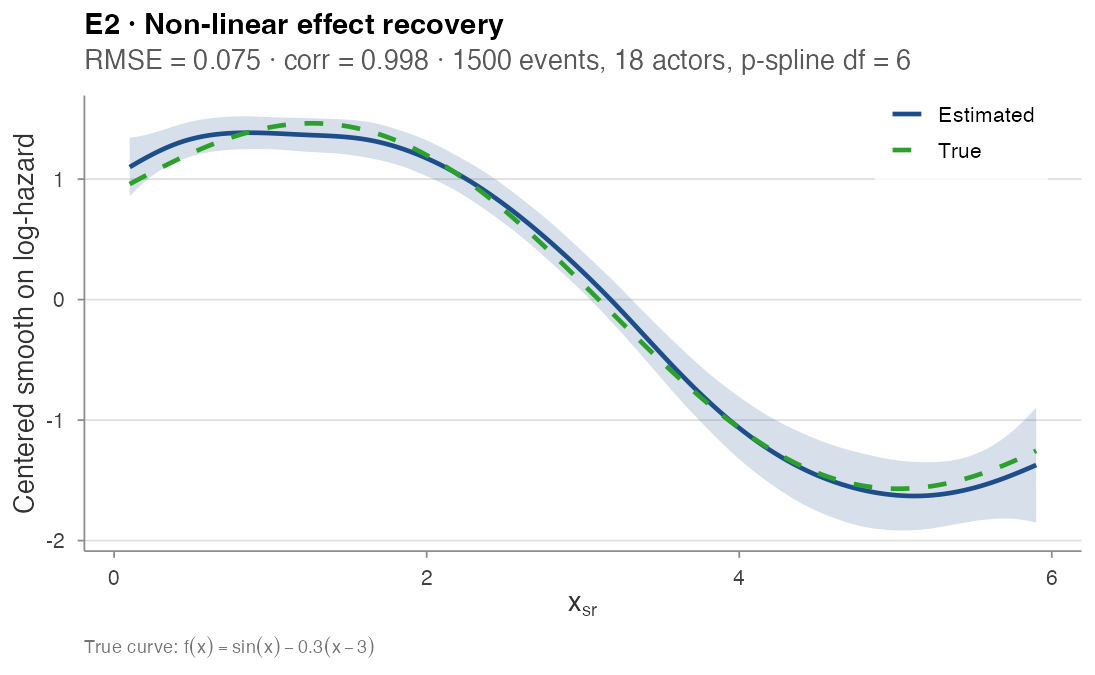
\includegraphics[width=0.7\textwidth]{figs/exp2-smooth.png}
\caption{E2 smooth recovery: the estimated penalized-spline partial effect
(with confidence band) overlaid on the true $f(x) = \sin(x) - 0.3(x-3)$;
centred RMSE $= 0.075$, correlation $= 0.998$.}
\label{fig:val-e2}
\end{figure}

\subsection{E3: Sender frailty under activity heterogeneity}
\label{sec:val-e3}

The third experiment asks whether strong per-sender activity heterogeneity
biases a fixed-coefficient \code{clogit} on \texttt{reciprocity\_count}, and
whether a Gamma sender frailty corrects any such bias. On a 20-actor network
with true $\beta = 0.5$ and three controls per case, per-sender baseline
offsets are injected through \texttt{contribution\_logits} rows under two
heterogeneity regimes: a \emph{strong} regime with lognormal activity
(median max/min ratio $\approx 84\times$, 2{,}500 events, 8 replicates) and
a \emph{mild} regime with $\mathrm{Gamma}(2,1)$ activity ($\approx 22\times$,
1{,}500 events, 10 replicates). Each replicate fits the naive
\code{clogit(event \textasciitilde{} reciprocity\_count + strata(stratum))}
against a \code{coxph} model adding \code{frailty(sender, "gamma")}.

\begin{table}[ht]
\centering
\caption{E3 sender frailty. The naive case-control estimator is robust to
$\approx 84\times$ sender-activity heterogeneity; the Gamma frailty adds
bias and variance rather than removing it.}
\label{tab:val-e3}
\begin{tabular}{llrrr}
\hline
Regime & Spec & mean $\hat\beta$ & SD & bias \\
\hline
strong ($\approx 84\times$) & naive clogit      & $0.498$ & $0.100$ & $-0.002$ \\
                            & $+$ sender frailty & $0.539$ & $0.110$ & $+0.039$ \\
mild ($\approx 22\times$)   & naive clogit      & $0.539$ & $0.086$ & $+0.039$ \\
                            & $+$ sender frailty & $0.554$ & $0.140$ & $+0.054$ \\
\hline
\end{tabular}
\end{table}

The hypothesized failure mode does not manifest
(Table~\ref{tab:val-e3}). The naive case-control estimator is robust to
sender-activity heterogeneity: in the strong regime it is essentially
unbiased ($-0.002$). Adding the Gamma frailty reduces bias in neither
regime; it introduces a small upward bias and inflates the variance, and
every frailty fit emitted inner-loop convergence warnings. The reason is
structural: the stratified case-control likelihood already conditions on the
stratum, which absorbs the per-sender baseline, so an extra frailty term has
nothing to correct and only injects noise. This \textbf{revises an earlier
reading} of the experiment, which had expected the frailty to be needed and
judged the design under-powered. With the stronger design, the conclusion is
that the correction is unnecessary in this setting
(Figure~\ref{fig:val-e3}).

\begin{figure}[ht]
\centering

\includegraphics[width=0.8\textwidth]{figs/exp3-frailty.png}
\caption{E3 frailty estimates: naive versus frailty-corrected $\hat\beta$
across replicates and regimes; the naive estimator centers on the truth.}
\label{fig:val-e3}
\end{figure}

\subsection{E4: Simulator wall-clock scaling}
\label{sec:val-e4}

The fourth experiment compares the two simulation kernels. The Gillespie
scheme is exact but processes one event at a time, recomputing the full risk
set per event; the $\tau$-leap scheme bundles events into fixed time slices
and should scale better for large actor universes. A
$4 \times 5 \times 2$ grid varies
\code{n\_actors} $\in \{15, 30, 60, 100\}$,
\code{n\_events} $\in \{500, 1000, 2500, 5000, 10000\}$, and
\code{method} $\in \{$\texttt{gillespie}, \texttt{tau\_leap}$\}$
($\tau = 0.05$), with a single reciprocity term at $\beta = 0.4$ and no
case-control sampling so wall-clock isolates the simulator. Absolute seconds
are machine-specific (Apple Silicon M1 Max); the scaling shape and the
ratios are what transfer.

\begin{table}[ht]
\centering
\caption{E4 simulator timings (stable cells). The $\tau$-leap kernel is
22--42$\times$ faster at \code{n\_actors} $= 60$ and up to
$\approx 100\times$ faster at \code{n\_actors} $= 100$.}
\label{tab:val-e4}
\begin{tabular}{rrrrr}
\hline
\code{n\_actors} & \code{n\_events} & Gillespie (s) & $\tau$-leap (s) & speedup \\
\hline
60  & 500    & $0.044$ & $0.002$ & $22\times$ \\
60  & 1{,}000  & $0.097$ & $0.003$ & $32\times$ \\
60  & 2{,}500  & $0.281$ & $0.008$ & $35\times$ \\
60  & 5{,}000  & $0.673$ & $0.016$ & $42\times$ \\
100 & 500    & $0.110$ & $0.003$ & $37\times$ \\
100 & 2{,}500  & $0.620$ & $0.009$ & $73\times$ \\
100 & 5{,}000  & $1.50$  & $0.018$ & $\approx 80\times$ \\
100 & 10{,}000 & $3.40$  & $0.033$ & $\approx 100\times$ \\
\hline
\end{tabular}
\end{table}

Table~\ref{tab:val-e4} reports the stable cells. The $\tau$-leap kernel is
22--42$\times$ faster at \code{n\_actors} $= 60$ and from 37$\times$ to
$\approx 100\times$ faster at \code{n\_actors} $= 100$, the gap widening
with \code{n\_events}. The honest counterpart is a shared failure map at
\emph{small} actor universes under this strongly self-exciting reciprocity
process: both back-ends break down, for opposite reasons. Gillespie's
per-dyad softmax underflows (``too few positive probabilities'') at
\code{n\_actors} $\in \{15, 30\}$ for \code{n\_events} $\ge 5000$ (and at 60
for 10{,}000 events), while $\tau$-leap's intensities blow up into a memory
explosion (seed-dependent at small sizes; all replicates fail at
\code{n\_events} $= 10000$ for \code{n\_actors} $\le 60$). At 10{,}000
events only the 100-actor cell is clean for both methods. This is a real
limitation worth knowing when simulating small, strongly self-exciting
networks (Figure~\ref{fig:val-e4}).

\begin{figure}[ht]
\centering
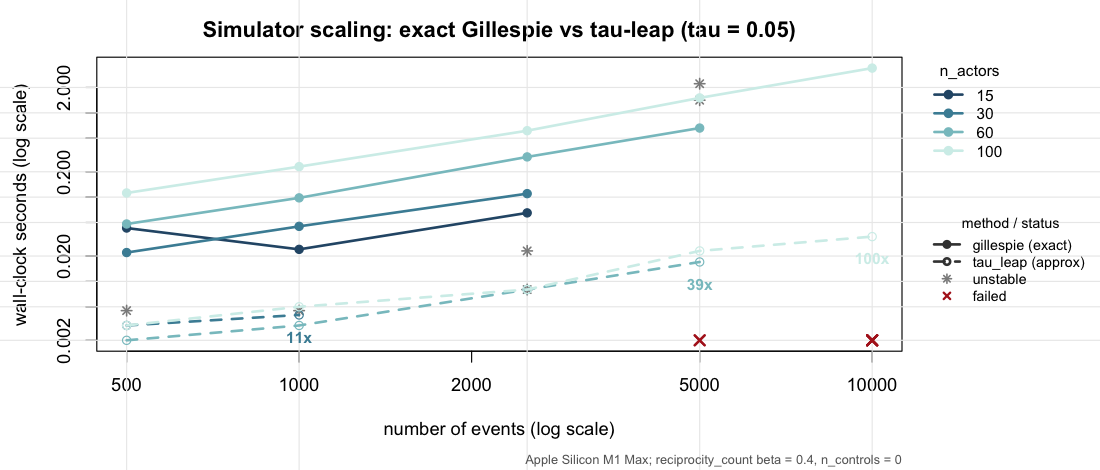
\includegraphics[width=0.8\textwidth]{figs/exp4-scaling.png}
\caption{E4 scaling lines: wall-clock seconds versus \code{n\_events} for
each kernel and actor count on log scales; $\tau$-leap stays an order of
magnitude or more below Gillespie in the stable cells.}
\label{fig:val-e4}
\end{figure}

\subsection{E5: Simulator/post-hoc engine parity}
\label{sec:val-e5}

The fifth experiment is the package's cross-implementation oracle. The
simulator records each endogenous statistic on the fly as it generates
events; the post-hoc engine \code{compute\_endogenous\_features()} re-derives
the same statistics from the timestamps alone. The two should agree
row-for-row on any case-control table the simulator emits. The design uses a
15-actor, 1{,}200-event simulation (one control per case; a 2{,}400-row
table) with 12 endogenous statistics active simultaneously across five
families and four variant axes, all C++-engine-supported. For each
statistic, \code{max |simulator - post-hoc|} is computed under two
conventions: a \emph{naive} recompute over the full case-control table, and
an \emph{aligned} recompute that passes \code{history\_log =} the realized
event rows, so that sampled controls neither pollute the running history nor
read post-update state at tied timestamps.

\begin{table}[ht]
\centering
\caption{E5 simulator/post-hoc parity. The naive recompute shows drift of
order \code{n\_events}; under \code{history\_log} alignment the engines agree
to floating-point precision.}
\label{tab:val-e5}
\begin{tabular}{lrr}
\hline
Statistic & naive (no \code{history\_log}) & aligned (\code{history\_log} $=$ events) \\
\hline
\texttt{reciprocity\_count}           & $12.0$ & $0$ \\
\texttt{transitivity\_count}          & $9.0$  & $0$ \\
\texttt{cyclic\_count}                & $10.0$ & $0$ \\
\texttt{sending\_balance\_count}      & $9.0$  & $0$ \\
\texttt{receiving\_balance\_count}    & $9.0$  & $0$ \\
\texttt{cyclic\_exp\_decay}           & $9.37$ & $4.3\times10^{-14}$ \\
\texttt{sending\_balance\_exp\_decay} & $8.67$ & $3.9\times10^{-14}$ \\
\texttt{transitivity\_time\_recent}   & $3.74$ & $0$ \\
\texttt{cyclic\_time\_recent}         & $3.74$ & $0$ \\
\texttt{receiving\_balance\_time\_first} & $0.70$ & $0$ \\
\texttt{reciprocity\_binary}          & $1.0$  & $0$ \\
\texttt{transitivity\_binary}         & $1.0$  & $0$ \\
\hline
\end{tabular}
\end{table}

Parity holds, and the previously reported ``bug'' was a comparison artifact
(Table~\ref{tab:val-e5}). An earlier run read the naive column as evidence
of a ``state-update ordering bug'' and advised treating the post-hoc engine
as authoritative for count statistics. That conclusion is retracted. The
naive recompute lets sampled control rows write into the running history
(producing count and exp-decay drift of order \code{n\_events}) and lets
tied rows read post-update state (producing the timing drift). Passing
\code{history\_log} reproduces the simulator's exact semantics: the C++
engine processes rows in time groups, every row at a tied timestamp reads
before any write, and only event rows write. Under that alignment the engines
agree to floating-point precision, with maximum absolute difference
$4.3 \times 10^{-14}$ (the exp-decay residue being summation-order noise).
There is no ordering bug, and neither engine needs to be privileged over the
other. The episode is the value proposition of a cross-implementation oracle:
two independent implementations of the same statistics, held against each
other, both expose the alignment subtlety and certify its resolution
(Figure~\ref{fig:val-e5}).

\begin{figure}[ht]
\centering

\includegraphics[width=0.8\textwidth]{figs/exp5-parity.png}
\caption{E5 parity bars: per-statistic maximum absolute difference under the
naive and aligned recompute conventions; the aligned bars collapse to the
floating-point floor.}
\label{fig:val-e5}
\end{figure}

\subsection{E6: Neural backend gradient correctness and interaction recovery}
\label{sec:val-e6}

The final experiment validates the pure-R \texttt{nn} backend. Two
properties are tested: its hand-derived analytic gradients must match
numerical differentiation, and the fitted network must match a linear
conditional logit when the truth is linear while outperforming it when
effects interact in a way an additive model cannot represent. For the
gradient check, a 3-feature MLP on four strata is differentiated analytically
and by central finite difference. For recovery, 600 case-1-control strata are
generated, the event in each drawn by a softmax over a true score, under two
regimes: a \textbf{linear} truth $\eta = 1.5\,x_1$ and an
\textbf{interaction} truth $\eta = 2.5\,x_1 x_2$. Both
\code{rem(method = "nn")} and \code{rem(method = "clogit")} are fit, and
top-1 concordance (the fraction of strata whose observed event scores
highest) is compared.

The analytic and numerical gradients agree to
$\max|\text{analytic} - \text{numerical}| = 1.4 \times 10^{-10}$, confirming
the backprop derivation. The recovery results are shown in
Table~\ref{tab:val-e6}.

\begin{table}[ht]
\centering
\caption{E6 interaction recovery (in-sample top-1 concordance). The neural
backend matches the linear conditional logit on a linear truth and recovers
the interaction structure where the additive model cannot.}
\label{tab:val-e6}
\begin{tabular}{lrr}
\hline
Truth & \code{clogit} (linear) & \code{nn} (MLP) \\
\hline
$\eta = 1.5\,x_1$ (linear)        & $0.78$ & $0.78$ \\
$\eta = 2.5\,x_1 x_2$ (interaction) & $0.52$ & $0.81$ \\
\hline
\end{tabular}
\end{table}

Under the linear truth the neural backend matches the linear conditional
logit (0.78 versus 0.78, with no overfitting penalty); under the interaction
truth, where the additive \code{clogit} is stuck near chance (0.52), the
joint MLP recovers the structure (0.81). We emphasize that these concordance
figures are \textbf{in-sample}: the metric is the network's own training-set
concordance, the \texttt{nn} backend reports no uncertainty quantification,
and factor predictors are not supported. The learned score surface
(Figure~\ref{fig:val-e6}, right) reproduces the saddle of $2.5\,x_1 x_2$ ---
high at the matching-sign corners, low at the opposite-sign corners. This is
precisely the regime the neural backend targets: when endogenous effects
interact, the additive backends cannot represent the structure, whereas an
MLP that scores the full candidate vector jointly can. This is an
accessibility and engineering contribution, not a claim of priority: neural
relational-event and temporal-point-process models are established prior art,
including STREAM's large-scale additive splines \citep{filippimazzola2024},
RMTPP \citep{du2016}, and the neural Hawkes process \citep{mei2017}.

\begin{figure}[ht]
\centering
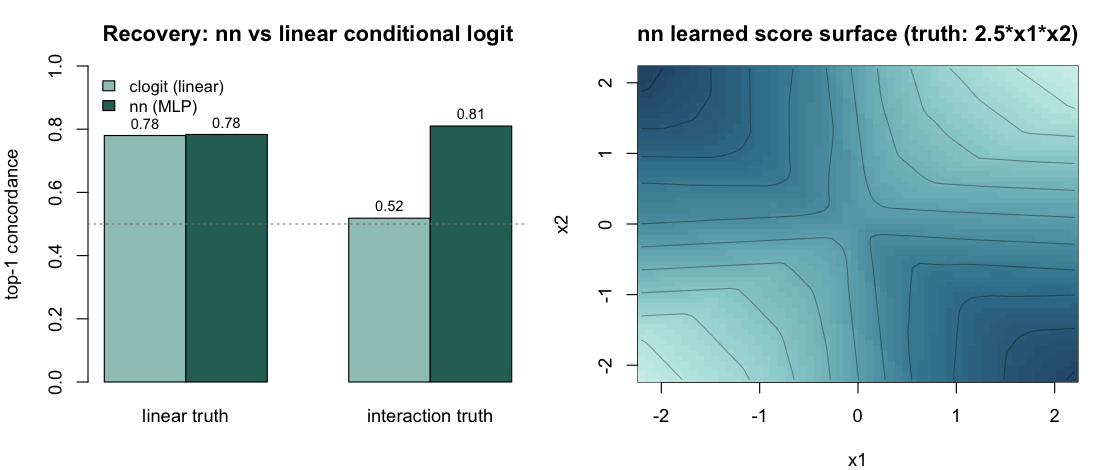
\includegraphics[width=0.9\textwidth]{figs/exp6-nn.png}
\caption{E6 neural backend. Left: in-sample top-1 concordance of \code{nn}
versus \code{clogit} under the linear and interaction truths. Right: the
learned score surface over $(x_1, x_2)$, reproducing the saddle of the
$2.5\,x_1 x_2$ interaction.}
\label{fig:val-e6}
\end{figure}

\subsection{E7: Additive-spline backend recovery, mini-batch invariance, and scaling}
\label{sec:val-e7}

The additive-spline architecture of Section~\ref{sec:framework-nn-additive}
--- per-covariate B-spline expansions trained by stochastic gradient on the
exact case-control partial likelihood, the STREAM construction of
\citet{filippimazzola2024} --- is checked on three properties: recovery of
additive effect shapes, invariance to mini-batching, and scaling against the
in-memory \code{gam} backend. The data-generating intensity is additive,
$\eta = \sin(2x_1) + 0.8\,x_2 + 0 \cdot x_3$, combining a nonlinear, a linear,
and a null effect, with one event and one sampled control per stratum.

Over ten Monte-Carlo replicates of $2{,}000$ strata
(Table~\ref{tab:val-e7-recovery}), the fitted curves recover the nonlinear and
linear effects (correlation $0.97$--$0.99$ with the centered truth) while the
null effect stays near-flat (amplitude $\approx 0.17$ against a unit-scale
signal). The fit is essentially identical under full-batch and mini-batch
training (\code{batch\_strata} of 256 and 64), and the additive-spline backend
improves top-1 concordance over the linear conditional logit ($0.74$ versus
$0.68$) by capturing the $\sin$ curvature the linear fit cannot represent
(Figure~\ref{fig:val-e7}, left).

\begin{table}[ht]
\centering\small
\begin{tabular}{lrrrr}
\toprule
Training & cor$(\hat f_1,\sin)$ & cor$(\hat f_2,\mathrm{lin})$ & null $\max|\hat f_3|$ & concordance \\
\midrule
full-batch & 0.974 & 0.994 & 0.176 & 0.739 \\
mini-batch (256) & 0.978 & 0.997 & 0.153 & 0.740 \\
mini-batch (64)  & 0.976 & 0.996 & 0.186 & 0.740 \\
linear \code{clogit} & --- & --- & --- & 0.676 \\
\bottomrule
\end{tabular}
\caption{E7 recovery and mini-batch invariance, averaged over ten replicates.}
\label{tab:val-e7-recovery}
\end{table}

On scaling (single fit at $2$k--$64$k strata), the additive-spline SGD is
faster and lighter than the \code{gam} fit on identical data, the gap widening
with size: at $64{,}000$ strata it runs in $8.1$\,s and $342$\,MB against the
\code{gam} backend's $12.7$\,s and $402$\,MB (Figure~\ref{fig:val-e7}, right).
This is the regime STREAM targets, here measured at modest scale on commodity
hardware; absolute timings are machine-dependent and were corroborated on a
second host.

\begin{figure}[ht]
\centering
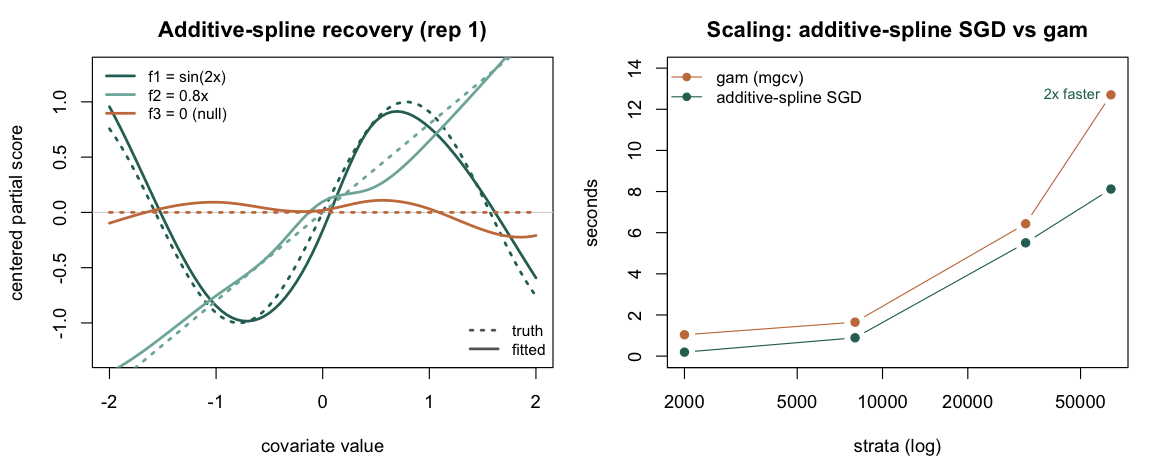
\includegraphics[width=\textwidth]{figs/exp7-additive.png}
\caption{E7 additive-spline backend. Left: fitted partial-effect curves
(solid) against the centered truths (dotted) for the nonlinear, linear, and
null covariates. Right: wall-clock scaling of additive-spline stochastic
gradient against the \code{gam} backend on the same case-control table.}
\label{fig:val-e7}
\end{figure}

Taken together, E1--E7 certify the simulator/likelihood consistency for
linear and smooth effects (E1, E2), the robustness of the naive
case-control estimator to actor-activity heterogeneity (E3), the relative
scaling and the honest failure boundaries of the two simulation kernels
(E4), the exact agreement of the simulator and post-hoc statistics engines
under correct history alignment (E5), and the correctness and
interaction-recovery behavior of the neural backend (E6), and the recovery, mini-batch invariance, and favorable scaling of the additive-spline backend against the in-memory smooth fit (E7). The two corrected
findings (E3 and E5) are reported in full because the test infrastructure
that produced the corrections --- the 48-file, $\sim$3{,}280-assertion suite
and the cross-implementation oracle --- is part of what \pkg{amore} offers.
